\chapter{外文资料的调研阅读报告或书面翻译}
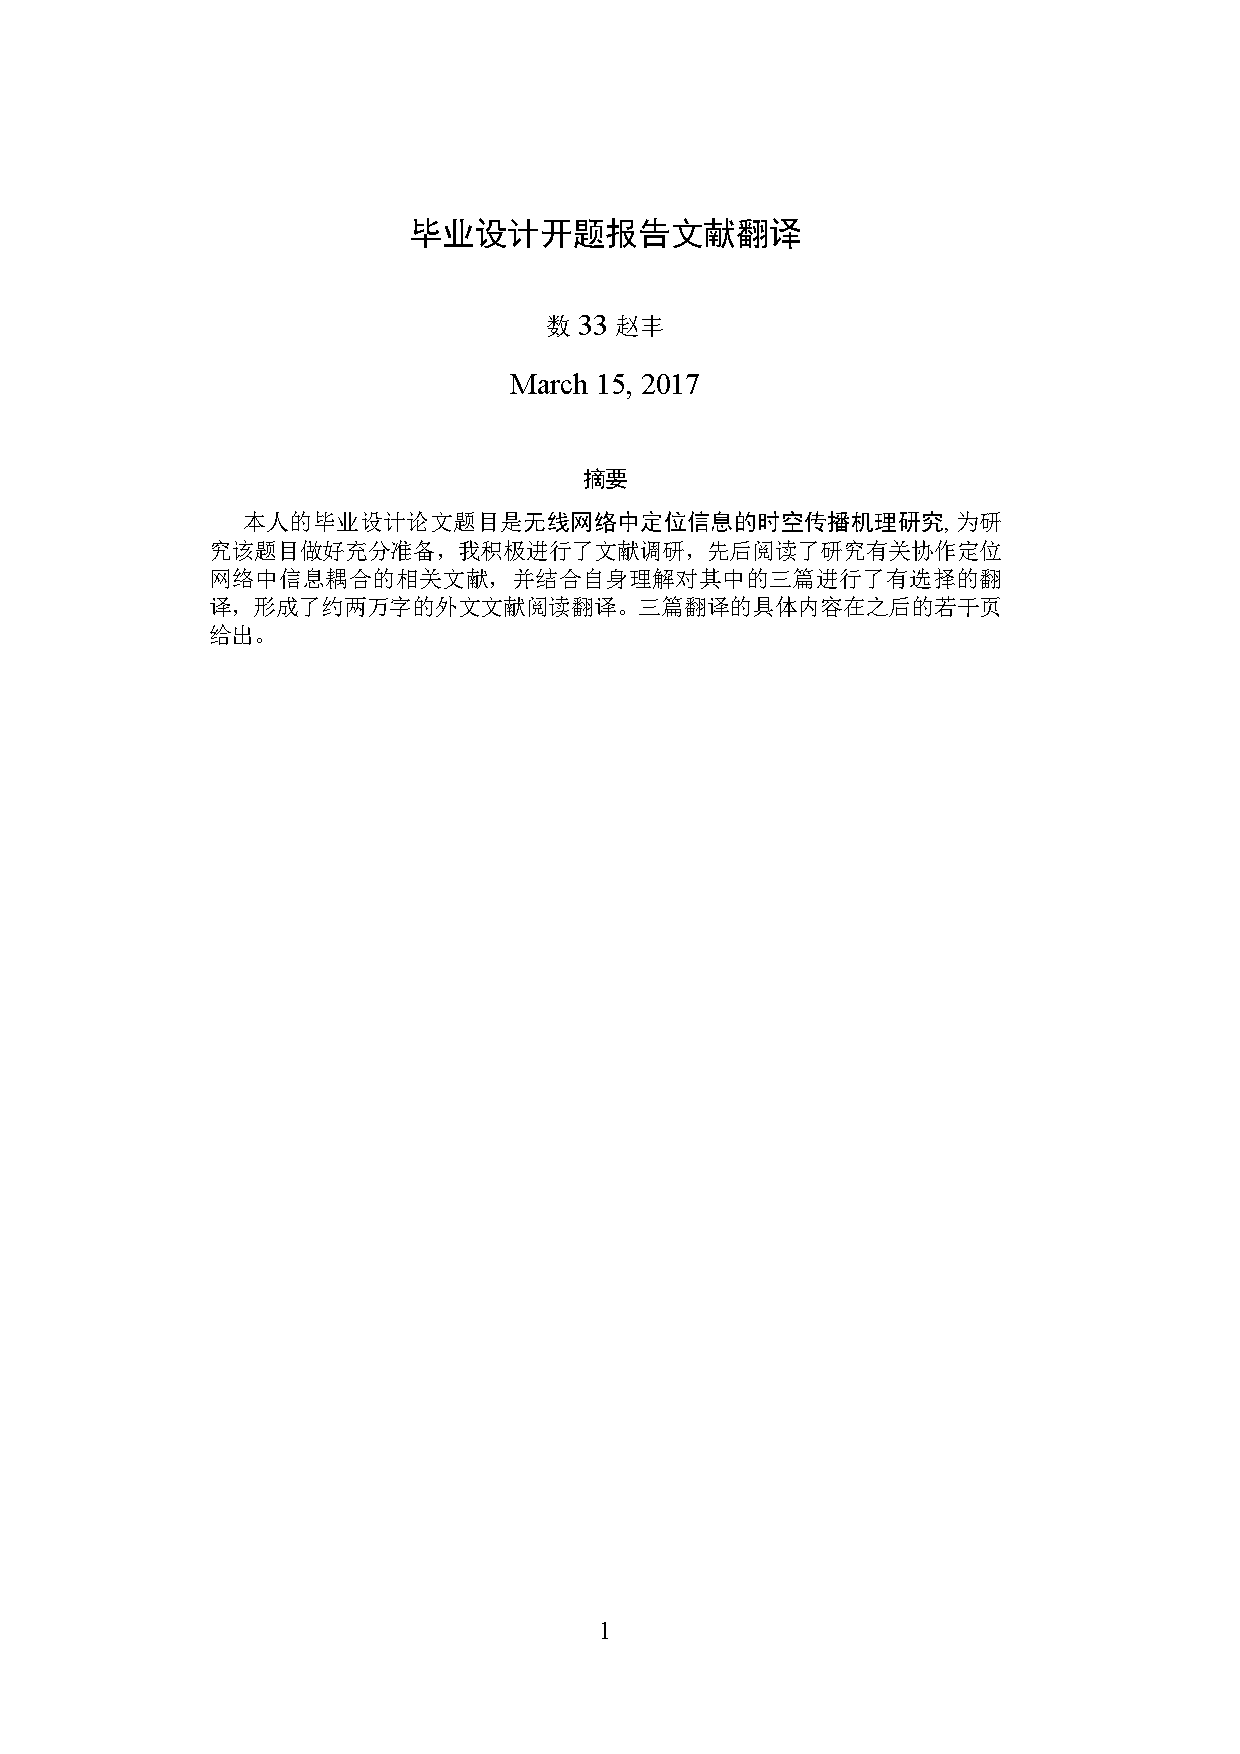
\includepdf[pages=-]{translation.pdf}
\chapter{公式的推导}
\section{建模过程的一些推导过程}
\subsection{定位问题中费舍尔信息矩阵一般结构推导}\label{A_F_1}
在非协作单节点定位中,测量量的联合概率分布由式(\ref{eq:single})给出,费舍尔信息矩阵是费舍尔信息量的自然推广,在满足一定正则性的条件下,费舍尔信息矩阵可以写成:
\begin{equation}
I(\bm{p})=-\mathbb{E}_{\bm{x}}(\bigtriangledown_{\bm{p}} \log f(\vec{x}|\bm{p}))^T(\bigtriangledown_{\bm{p}} \log f(\vec{x}|\bm{p}))
\end{equation}
其中f是随机向量$\vec{x}$的密度函数,利用上面的公式,首先对式(\ref{eq:single})取对数并求梯度得:
\begin{equation}
\bigtriangledown_{\bm{p}}\ln f=-\sum_{i=1}^{N_b}\frac{||\bm{p}_i^b-\bm{p}||-x_i}{\sigma_i^2}\frac{\bm{p}^b_i-\bm{p}}{||\bm{p}^b_i-\bm{p}||}.
\end{equation}
注意到$\frac{||\bm{p}_i^b-\bm{p}||-x_i}{\sigma_i}\sim N(0,1)$,所以按照费舍尔信息矩阵的定义可得到式(\ref{eq:uu})的结果。
\section{研究成果的一些推导过程}
\subsection{两个未知节点协作最小误差界的一个充分条件}\label{B_F_0}
由式(\ref{eq:4_characteristic_polynomial}),SPEB为其所有根的倒数和,因此具有如下形式
\begin{equation}\label{eq:SPEB_GLOBAL}
\text{SPEB}=\frac{\displaystyle\sum \frac{1}{\lambda_i}+\epsilon(\frac{\cos^2(\theta)}{\lambda_1}(\sum_{i \neq 1}\frac{1}{\lambda_i})+\frac{\sin^2(\theta)}{\lambda_2}(\displaystyle\sum_{i \neq 2}\frac{1}{\lambda_i})+\frac{\cos^2(\phi)}{\lambda_3}(\sum_{i \neq 3}\frac{1}{\lambda_i})+\frac{\sin^2(\phi)}{\lambda_4}(\sum_{i \neq 4}\frac{1}{\lambda_i}))}{\displaystyle 1+\epsilon(\frac{\cos^2(\theta)}{\lambda_1}+\frac{\sin^2(\theta)}{\lambda_2}+\frac{\cos^2(\phi)}{\lambda_3}+\frac{\sin^2(\phi)}{\lambda_4})}
\end{equation}
对固定的$\phi$,我们证明SPEB关于$\theta$是单调递减的。记$k=\frac{\cos^2 \theta}{a_1}+\frac{\sin^2 \theta}{a_2}$,$u=(\frac{1}{a_3}+\frac{1}{a_4}),v=(\frac{1}{a_1}+\frac{1}{a_2})$.~(\ref{eq:SPEB_GLOBAL})可以化为:
\begin{equation}
\text{SPEB}=u\frac{1+(\frac{1}{a_1}+\frac{1}{a_2})/u+\epsilon(\frac{1}{a_1a_2 u}+\frac{1}{a_3a_4 u}+k+(\frac{\cos^2\phi}{a_3}+\frac{\sin^2\phi}{a_4})\frac{v}{u})}{1+\epsilon(k+(\frac{\cos^2\phi}{a_3}+\frac{\sin^2\phi}{a_4}))}.
\end{equation}
SPEB可以写成关于k的反比例函数$u\frac{A+k}{B+k}$的形式,其中
\begin{align}\notag
A=&(1+(\frac{1}{a_1}+\frac{1}{a_2})/u)/\epsilon+\frac{1}{a_1a_2 u}+\frac{1}{a_3a_4 u}+(\frac{\cos^2\phi}{a_3}+\frac{\sin^2\phi}{a_4})\frac{v}{u}\\
B=&1/\epsilon+(\frac{\cos^2\phi}{a_3}+\frac{\sin^2\phi}{a_4}).
\end{align}
如果能证明$A \geq B$,那么该反比例函数关于k是单调递减的。
\begin{align}\notag
A-B=&(\frac{1}{a_1}+\frac{1}{a_2})/u\epsilon+\frac{1}{a_1a_2 u}+\frac{1}{a_3a_4 u}+(\frac{\cos^2\phi}{a_3}+\frac{\sin^2\phi}{a_4})(\frac{v}{u}-1)\\
\geq &\frac{1}{a_3a_4 u}+(\frac{\cos^2\phi}{a_3}+\frac{\sin^2\phi}{a_4})(\frac{v}{u}-1)\\
=&\frac{1}{u}((\frac{1}{a_1}+\frac{1}{a_2})(\frac{\cos^2\phi}{a_3}+\frac{\sin^2\phi}{a_4})-(\frac{\cos^2\phi}{a_3^2}+\frac{\sin^2\phi}{a_4^2})).\notag
\end{align}
由假设:$\frac{1}{a_1}+\frac{1}{a_2}\geq \max\{\frac{1}{a_4},\frac{1}{a_3}\}$,
所以$A-B\geq 0$。
\begin{equation}
k=\frac{1}{a_1}+\sin^2 \theta(\frac{1}{a_2}-\frac{1}{a_1}).
\end{equation}
根据上式,和假设条件$a_1\geq a_2$,可得在$\sin^2(\theta)\in[0,1]$的区间内k关于$\sin^2(\theta)$是单调递增的。所以由复合函数的单调性,SPEB关于$\theta$是单调递减的。
同理可证明条件$\frac{1}{a_3}+\frac{1}{a_4}\geq \max\{\frac{1}{a_1},\frac{1}{a_2}\}$是保证固定$\theta$的情况下SPEB关于$\phi \in [0,\frac{\pi}{2}]$是单调递减的。
\subsection{单节点动态定位问题等效费舍尔信息矩阵推导}\label{B_F_1}
为简化符号,记$\bm{u}:=\bm{u}_{N_a-1}$,2阶单位阵记为$\bm{I}_2$,由等效费舍尔信息矩阵的定义,有
\begin{align}\notag\label{eq:initial_efim}
  U_{N_a}=&\lambda \bm{I}_2+\bm{u}\bm{u}^T-\bm{u}\bm{u}^T U_{N_a-1}^{-1}\bm{u}\bm{u}^T\\
  =&\lambda \bm{I}_2+(1-\bm{u}^T U_{N_a-1}^{-1}\bm{u})\bm{u}\bm{u}^T.
\end{align}
因为$\bm{u}\bm{u}^T=U\begin{pmatrix}
                     1 & 0 \\
                     0 & 0
                   \end{pmatrix}U^{-1}$,其中$U$是由$\bm{u}$的方向角确定的二维旋转矩阵,所以
$U_{N_a}$相似于下面的矩阵
\begin{equation}
U_{N_a}\sim \begin{pmatrix}
                           \lambda+1-\bm{u}^T U_{N_a-1}^{-1}\bm{u} & 0 \\
                           0 & \lambda
                         \end{pmatrix}.
\end{equation}

我们定义$T_i=\lambda+1-\bm{u}^T U_{N_a-i}^{-1}\bm{u}$并设$U_{N_a-1}=\bm{u}\bm{u}^T+J_2$
由式(\ref{eq:woodbury})可得
\begin{align}\notag
T_1=&\lambda+1-\bm{u}^T (\bm{u}\bm{u}^T+J_2)^{-1}\bm{u}\\
=&\lambda+(1+\bm{u}^T J_2^{-1}\bm{u})^{-1}.
\end{align}
进一步设$v:=\bm{u}_{N_a-2}$,则$J_2=\lambda \bm{I}_2+(1-\bm{v}^T U_{N_a-2}^{-1}\bm{v})\bm{v}\bm{v}^T=V\begin{pmatrix}
                     \lambda+1-\bm{v}^T U_{N_a-2}^{-1}\bm{v} & 0 \\
                     0 & \lambda
                   \end{pmatrix}V^{-1}$
设$\bm{u}=(\cos\phi_1,\sin\phi_1)^T,\bm{v}=(\cos\phi_2,\sin\phi_2)^T$,则
\begin{equation}
V^{-1}\bm{u}=\begin{pmatrix}
                     \cos\phi_2 & \sin\phi_2 \\
                     -\sin\phi_2 & \cos\phi_2
                   \end{pmatrix}\binom{\cos\phi_1}{\sin\phi_1}=\binom{\cos(\phi_1-\phi_2)}{\sin(\phi_1-\phi_2)}=:w.
\end{equation}
所以
\begin{align*}
T_1=&\lambda+(1+\bm{w}^T \begin{pmatrix}
                     \lambda+1-\bm{v}^T U_{N_a-2}^{-1}\bm{v} & 0 \\
                     0 & \lambda
                   \end{pmatrix}^{-1}\bm{w})^{-1}\\
                   =&\frac{1}{1+\cfrac{\cos^2(\phi_1-\phi_2)}{T_2}+\cfrac{\sin^2(\phi_1-\phi_2)}{\lambda}}.
\end{align*}
递推可得一般形式。
终止条件:
\begin{align*}
T_{N_a-1}&=\lambda+1-\bm{u}_1^T(\lambda\bm{I}+\bm{u}_1\bm{u}_1^T)^{-1}\bm{u}_1\\
&=\lambda+\cfrac{1}{\lambda+\cfrac{1}{\lambda}}.
\end{align*}
\subsection{定理\ref{theorem:arbitrary_curve}的证明}\label{B_F_6}
式(\ref{eq:starting_or_ending})给出了式(\ref{eq:limiting_cf})右端是$\bm{p}(t)$为直线的情形。由于对于任意的平面曲线和角度序列$\{\theta_i\}$,$T_1(N_a)$是关于$N_a$的增函数且小于$\lambda+1$,因此式(\ref{eq:limiting_cf})左端的极限总是存在的。
考虑由$\bm{p}(t)$确定的角度序列$\{\theta_i\}$以如下的方式趋近于直线对应的直线序列:
\begin{equation}
\{\theta_1,\theta_2,\theta_3,\dots\}\rightarrow\{0,\theta_2,\theta_3,\dots\}\rightarrow
\{0,0,\theta_3,\dots\}\rightarrow\dots
\end{equation}
记将前n个角度置零后由式(\ref{eq:recursive_efim})确定的连分式为$K_n$,我们首先给出:
\begin{equation}\label{eq:arbitrary_curve_1}
\lim_{n\to\infty}K_n=\frac{\lambda+\sqrt{4\lambda+\lambda^2}}{2}
\end{equation}
为证式(\ref{eq:arbitrary_curve_1}),记角度序列$\{0,0,\dots,\theta_{n+1},\dots,\}$去掉前r项后对应的连分式为$K^r_n$
\begin{align}\notag
|K_n-M^*|=&\frac{|\frac{1}{M^*}-\frac{1}{K^2_n}|}{(1+\frac{1}{M^*})(1+\frac{1}{K^2_n})}\\
\leq &|\frac{1}{M^*}-\frac{1}{K^2_n}|\notag\\
= &\frac{|\frac{1}{M^*}-\frac{1}{K^3_n}|}{K^2_n(M^*+1)(1+\frac{1}{K^3_n})}\\
=& \frac{|\frac{1}{M^*}-\frac{1}{K^3_n}|}{(M^*+1)(\lambda+1+\frac{1}{K^3_n+1})}\notag\\
\leq & \frac{|\frac{1}{M^*}-\frac{1}{K^3_n}|}{(\lambda+1)^2}.\notag
\end{align}
当$r<n$ 时,
\begin{equation}
|\frac{1}{M^*}-\frac{1}{K^r_n}|\leq \frac{|\frac{1}{M^*}-\frac{1}{K^{r+1}_n}|}{(\lambda+1)^2}.
\end{equation}
因此:
\begin{equation}
|K_n-M^*|\leq \frac{|\frac{1}{M^*}-\frac{1}{K^{n}_n}|}{(\lambda+1)^{2(n-2)}}.
\end{equation}
故式(\ref{eq:arbitrary_curve_1})成立。
补充定义$K_0=\lim_{\Delta t\to 0}T_1(N_a)$这样式(\ref{eq:limiting_cf})即等价为
\begin{equation}\label{eq:equivalent_limiting_cf}
\sum_{i=1}^{\infty}(K_{i-1}-K_{i})=0.
\end{equation}
先考虑$K_0-K_1$,二者的差别是$\theta_1$是否为0,
\begin{align}\notag
K_0-K_1=&\frac{1}{1+\frac{1}{K_1^1}}-\frac{1}{1+\frac{1}{K_1^1}+\sin^2\theta_1(\frac{1}{\lambda}-\frac{1}{K_1^1})}\\
\leq & (\frac{1}{\lambda}-\frac{1}{K_1^1})\sin^2\theta_1.
\end{align}
类似式(\ref{eq:arbitrary_curve_1})的推导:
\begin{equation}
K_r-K_{r+1}\leq \sin^2\theta_{r+1}(\frac{1}{\lambda}-\frac{1}{K_{r+1}^{r+1}})\frac{1}{(\lambda+1)^{2r}}.
\end{equation}
由条件$\bm{p}'(t)$存在且连续可得切向量是连续变化的,由微分中值定理在闭区间内存在常数c使得角度变化量$\theta_i\leq c\Delta t$。
由正弦函数的单调性推出:
\begin{equation}
K_r-K_{r+1}\leq \sin^2 (c\Delta t) \frac{1}{\lambda}\frac{1}{(\lambda+1)^{2r}}.
\end{equation}
因此
\begin{equation}\label{eq:quatratic_convergence}
0\leq \sum_{i=1}^{N_a}(K_{i-1}-K_{i})\leq \sin^2 (c\Delta t) \frac{1}{\lambda}\sum_{i=1}^{\infty}\frac{1}{(\lambda+1)^{2i}}.
\end{equation}
无穷级数$\sum_{i=1}^{\infty}\frac{1}{(\lambda+1)^{2i}}$收敛,所以当$\Delta t\to 0$时$N_a\to \infty$,式(\ref{eq:equivalent_limiting_cf})成立。

\subsection{单节点动态定位问题等效费舍尔信息衰减上下界}\label{B_F_2}
为记号简便记$T'_1=T_1(N_a+1),T_1=T_1(N_a)$
%考虑在原有基础上增加一层节点,
%于是协作层数由原来的$N_a-1$变为$N_a$。等效费舍尔信息矩阵较大的特征值分别记为$T_1,T'_1$,
为便于比较,我们在$T_1$中引入虚拟节点将其层数也拓展为$N_a$,它只有锚点的定位信息,这样它们的区别是连分式的末端$T_{N_a}=\lambda$,$T'_{N_a}=\lambda+\frac{1}{1+1/\lambda}$
对$|T_1-T'_1|$从外向里通分得:
\begin{align}\notag
|T_1-T'_1|=&\frac{|\frac{1}{T_2}-\frac{1}{T'_2}|\cos^2\theta_1}{(1+\frac{\sin^2\theta_1}{\lambda}+\frac{\cos^2\theta_1}{T_2})
(1+\frac{\sin^2\theta_1}{\lambda}+\frac{\cos^2\theta_1}{T'_2})}\\
\leq &|\frac{1}{T_2}-\frac{1}{T'_2}|.
\end{align}
继续放缩$|\frac{1}{T_2}-\frac{1}{T'_2}|$有:
\begin{align}\notag
|\frac{1}{T_2}-\frac{1}{T'_2}|= & \frac{|\frac{1}{T_3}-\frac{1}{T'_3}|\cos^2\theta_2}{(1+\lambda(1+\frac{\sin^2\theta_2}{\lambda}+\frac{\cos^2\theta_2}{T_3}))
(1+\lambda(1+\frac{\sin^2\theta_2}{\lambda}+\frac{\cos^2\theta_2}{T'_3}))}\\
\leq & |\frac{1}{T_3}-\frac{1}{T'_3}|\frac{1}{(1+\lambda)^2}.
\end{align}
逐次递推得
\begin{equation}
|T_1-T'_1|\leq \frac{1}{(1+\lambda)^{2(N_a-2)}} |\frac{1}{T_{N_a}}-\frac{1}{T'_{N_a}}|.
\end{equation}
而:
\begin{equation}
|\frac{1}{T_{N_a}}-\frac{1}{T'_{N_a}}|=\frac{1}{\lambda^2+2\lambda}.
\end{equation}
对于下界,因为$T_2,T'_2\geq \lambda$
\begin{equation}
|T_1-T'_1|\geq \frac{\cos^2\Delta\theta|\frac{1}{T_2}-\frac{1}{T'_2}|}{(1+1/\lambda)^2}.
\end{equation}
\begin{equation}
|\frac{1}{T_2}-\frac{1}{T'_2}|\geq \frac{\cos^2\Delta\theta|\frac{1}{T_3}-\frac{1}{T'_3}|}{(2+\lambda)^2}
\end{equation}
逐次递推得下界。
%\subsection{推论\ref{corollary:exponential_decreasing}的证明}\label{B_F_5}
%由定理\ref{theorem:exponential_decreasing}的结论:
%\begin{equation}
%T_{N_a}=\sum_{k=1}^{N_a-1}\Delta_{+}T_k
%\end{equation}
%因此当$N_a\geq 2$时
%\begin{equation}
%|T_{N_a}-T_{\infty}|=\sum_{k=N_a}^{\infty}\Delta_{+}T_k\leq %\frac{1}{\lambda^2+2\lambda}\sum_{k=N_a}^{\infty}\frac{1}{(\lambda+1)^{2(k-2)}}=\frac{1}{(\lambda^2+2\lambda)^2}\frac{1}{(\lambda+1)^{2(N_a-3)}}
%\end{equation}
%取$q=(\lambda+1)^2$,其余常数为C即可。
\subsection{单节点非均一测距误差等效费舍尔信息矩阵推导}\label{B_F_3}
类似式(\ref{eq:initial_efim})有:
\begin{equation}
U_{N_a}=\bm{I}+(\lambda_1-\lambda_1^2 \bm{u}^T U_{N_a-1}^{-1}\bm{u})\bm{u}\bm{u}^T.
\end{equation}
而
\begin{equation}
T_1=1+\lambda_1-\lambda_1^2 \bm{u}^T U_{N_a-1}^{-1}\bm{u}=1+(\lambda_1^{-1}+\bm{u}^T\bm{J}_2^{-1}\bm{u})^{-1}.
\end{equation}
对$J_2=\bm{I}_2+(\lambda_2-\lambda_2^2\bm{v}^T U_{N_a-2}^{-1}\bm{v})\bm{v}\bm{v}^T$提取关于$\bm{v}$的旋转矩阵即得到
式(\ref{eq:recursive_efim_second})。
另外从式(\ref{eq:recursive_efim_second})出发,设$\theta'_1\leq \theta_1$,作差:
\begin{equation}
T_1(\theta'_1)-T_1(\theta_1)=\frac{1}{A}(\cos^2\theta'_1-\cos^2\theta_1)(1-\frac{1}{T_2})\geq 0
\end{equation}
其中$A>0$,由上式可看出角度$\theta_1$越小$T_1$越大,同理$\theta_i$越小$T_i$越大,而由连分式的表达式可以看出$T_1$关于$T_2$递增,而连分式本身具有自相似性,因此诸$\theta_i$减小可以增大信息量$T_1$。

\subsection{引理~\ref{lemma:hexagon}的推导}\label{B_F_4}
  设式(\ref{eq:equiv})左边为B,$A=\lambda+\frac{3}{2}$,那么由Woodbury矩阵求逆公式有
  \begin{equation}
  (A+\frac{1}{\lambda+3/2-\frac{3/2}{\lambda+3/2}})^{-1}=A^{-1}-A^{-1}BA^{-1}.
  \end{equation}
  整理得:
  \begin{equation}
  B=A-\frac{A^2}{A+\frac{1}{\lambda+3/2-\frac{3/2}{\lambda+3/2}}}.
  \end{equation}
  通分化简得证。
\section{本文中用到的关于连分式的结论}\label{C_F}
\begin{definition}
  有限序列$t_1,t_2,\dots,t_r$满足$t_j\geq 1$对于$j\geq2$可以递推地定义有限连分式
  \begin{equation}
  [t_1,t_2,\dots,t_r]:=t_1+\frac{1} {[t_2,\dots,t_r]}.
  \end{equation}
\end{definition}
\begin{theorem}\label{thm:basic}
  设$p_j=t_j p_{j-1}+p_{j-2},q_j=t_j q_{j-1}+q_{j-2}$,$M_j=\left(\begin{matrix}p_j&p_{j-1}\\q_j&q_{j-1}\end{matrix}\right)$,
  $p_0,p_1,q_0,q_1$由$M_0=I_2$给出,且$T_j=\left(\begin{matrix}t_j&1\\1&0\end{matrix}\right)$则有下面三个恒等式:
  \begin{enumerate}
    \item $M_j=M_{j-1}T_j$,
    \item $\binom{p_j}{q_j}=(\prod_{i=1}^r T_i )\binom{1}{0}$,
    \item $[t_1,t_2,\dots,t_r]=\frac{p_r}{q_r}$.
  \end{enumerate}
\end{theorem}
\begin{theorem}\label{theorem:quadratic_cyclic}
若$\lim_{r\to \infty}[t_1,t_2,\dots,t_r]$存在,该极限是形如$\frac{a+b\sqrt{m}}{c}$的二次根式当且仅当序列$t_i$从某项开始是周期的,即$\exists c\text{和}r,\,s.t.\, t_{i}=t_{i+r},\forall i\geq c$。
\end{theorem}
\begin{remark}

对于定理\ref{theorem:quadratic_cyclic},$\lim_{r\to \infty}[t_1,t_2,\dots,t_r]$值可用二次方程不动点的方法求出\cite{ContinuedFraction}。
%设$\left(\begin{matrix}a&b\\c&d\end{matrix}\right)=(\prod_{i=1}^{rc} %T_{i+c})$,称$\left(\begin{matrix}a&b\\c&d\end{matrix}\right)$对应着分式线性变换K,如果$K(z)=\frac{az+b}{cz+d}$。
%可以证明系数为实数的分式线性变换以函数复合作为群运算与行列式为1的2阶方阵以矩阵乘积作为群运算是同构的。
%c之前的$t_i$对应着矩阵$T_i$的乘积矩阵看作分式线性变换F。可以进一步说明二次根式和T和F的有如下的关系:
%\begin{enumerate}
%  \item 首先求解$K$的不动点即解二次方程$x=\frac{ax+b}{cx+d}$得x
%  \item $F(x)=\lim_{r\to \infty}[t_1,t_2,\dots,t_r]$,F(x)即为极限$\lim_{r\to \infty}[t_1,t_2,\dots,t_r]$
%\end{enumerate}
%一般二次方程有两个根,而有限连分式的极限值是唯一的,这时可根据极限值介于序列的前两个数之间剔除一个不合理的不动点。
\end{remark}
